\documentclass[11pt, a4paper]{article}

% === PACKAGES ===
\usepackage[utf8]{inputenc}
\usepackage{amsmath}
\usepackage{graphicx}
\usepackage[margin=1in]{geometry} % Standard margin, guide only specifies A4.
\usepackage{setspace}
\usepackage{caption}
\usepackage{tikz}
\usetikzlibrary{shapes.geometric, arrows.meta, positioning, calc}
\usepackage{float}
\usepackage{booktabs}
\usepackage{kotex}
\usepackage{multirow}

% Page numbers at the bottom center.
\usepackage{fancyhdr}
\pagestyle{fancy}
\fancyhf{} % Clear all header and footer fields
\cfoot{\thepage}
\renewcommand{\headrulewidth}{0pt}
\renewcommand{\footrulewidth}{0pt}

% Double spacing for the main body.
\doublespacing

% Input the TikZ style definitions from your graph.tex file
\tikzset{
    title/.style={font=\Large\bfseries},
    block/.style={rectangle, rounded corners, text width=2.5cm, minimum height=1.5cm, text centered, draw=black, fill=gray!20, font=\small\setstretch{0.9}},
    space/.style={rectangle, rounded corners, minimum width=3.5cm, minimum height=3.5cm, draw=black!80, fill=gray!10, text centered, font=\small\setstretch{0.9}},
    output/.style={diamond, aspect=2, minimum size=1.0cm, text centered, draw=black, fill=gray!20, font=\small\setstretch{0.9}},
    main_arrow/.style={thick, -Triangle, line width=1pt},
    update_arrow/.style={thick, dashed, -Triangle, draw=red!80, rounded corners},
    sarc_emb/.style={circle, fill=red!60, draw=black, minimum size=8pt, inner sep=0pt},
    norm_emb/.style={rectangle, fill=blue!60, draw=black, minimum size=8pt, inner sep=0pt},
    force_arrow/.style={-stealth, dashed}
}

% === DOCUMENT START ===
\begin{document}

% Page numbering for Abstract in lowercase roman.
    \pagenumbering{roman}
    \setcounter{page}{1}

% --- COVER PAGE ---
    \begin{titlepage}
        \centering
        \vspace*{3cm}
        {\huge SimSCLSD: A Simple Framework for Supervised Contrastive Learning of Sarcasm Detection}

        \vspace{1cm}
        {\large 반어 표현 탐지를 위한 단순 지도 대조 학습 프레임워크}
        \vfill

        {\large 2025년 \quad 월}
        \vspace{1.5cm}

        {\large 서울대학교 공과대학} \\
        {\large 전기·정보공학부}

        \vspace{1cm}
        {\large 엄 태 윤}

    \end{titlepage}

% --- APPROVAL PAGE ---
    \begin{titlepage}
        \centering
        \vspace*{2cm}
        {\huge SimSCLSD: A Simple Framework for Supervised Contrastive Learning of Sarcasm Detection}

        \vspace{1cm}
        {\large 반어 표현 탐지를 위한 단순 지도 대조 학습 프레임워크}

        \vfill
        {\large 지도교수 심 규 석}

        \vspace{1cm}
        {\large 이 논문을 공학학사 학위논문으로 제출함}

        \vspace{0.5cm}
        {\large 2025년 \quad 월}

        \vspace{0.5cm}
        {\large 서울대학교 공과대학} \\
        {\large 전기·정보공학부}

        \vspace{0.5cm}
        {\large 엄 태 윤}

        \vspace{1.5cm}
        {\large 엄태윤의 학사 학위논문을 인준함}

        \vspace{0.5cm}
        {\large 2025년 \quad 월 \quad 일}

        \vspace{0.5cm}
        {\large 지도교수 \_\_\_\_\_\_\_\_\_\_ (인)}

    \end{titlepage}

% --- ABSTRACT ---
    \begin{center}
    {\Large\bfseries Abstract}
    \end{center}

    \vspace{1em}

    Sarcasm detection constitutes a pivotal challenge in Natural Language Processing (NLP) due to its ubiquity in online discourse and its tendency to invert the polarity of literal statements.
    Failing to detect sarcastic intent often results in significant errors in downstream tasks such as sentiment analysis and opinion mining.
    However, sarcasm is highly nuanced and context-dependent, making it difficult for standard classification models to identify accurately.
    While pre-trained Transformer-based language models have established standard baselines, they are typically fine-tuned using a Cross-Entropy (CE) loss.
    This approach may not be optimal for learning discriminative representations, especially for a nuanced task like sarcasm where the boundary between classes is subtle.

    To address this limitation, we present SimSCLSD, a Simple framework for Supervised Contrastive Learning of Sarcasm Detection, which introduces a two-stage training process.
    Contrastive learning is a paradigm that learns representations by contrasting positive pairs against negative pairs to induce a well-structured embedding space.
    In our first stage, we employ a supervised contrastive pre-training phase where a RoBERTa-based encoder is optimized to pull representations of same-label examples together while pushing apart representations of different-label examples.
    Unlike standard self-supervised contrastive methods that rely on data augmentation of a single instance, our approach leverages label information to utilize multiple positive samples within a batch.
    In the second stage, the model is fine-tuned with a standard CE loss to learn the final classification boundary.

    We evaluate our approach on the Reddit and Twitter datasets from the FigLang 2020 Sarcasm Detection shared task.
    Our experiments demonstrate that this contrastive pre-training step can effectively create more separable representations, showing its potential as an effective intermediate step for fine-tuning transformers on nuanced, context-dependent classification tasks.

    \vspace{2em}
    \noindent
    \textbf{keywords:} sarcasm detection, supervised contrastive learning, representation learning, text classification, conversational context, embedding space

    \vspace{1em}
    \noindent
    \textbf{Student Number: 2019-18535}

    \clearpage

% --- TABLE OF CONTENTS ---
    \tableofcontents

    \clearpage

% --- MAIN BODY ---
    \pagenumbering{arabic}
    \setcounter{page}{1}

    \section{Introduction}
    With the proliferation of social media platforms such as Twitter and Reddit, the volume of user-generated content has grown exponentially.
    This data offers immense potential for analyzing public opinion and sentiment.
    However, the informal nature of online discourse introduces significant noise, with figurative language---specifically sarcasm---posing a formidable barrier to accurate automated analysis~\cite{ghosh2020report}.
    Sarcasm is defined as a form of verbal irony where the speaker's intended meaning is often the opposite of the literal interpretation of their words.
    For instance, the phrase ``Great weather we're having'' spoken during a storm conveys a negative sentiment despite the positive adjective ``Great.''
    Consequently, failure to detect sarcasm can result in the complete inversion of a sentiment analysis system's prediction, rendering it unreliable for real-world applications.

    The primary difficulty in sarcasm detection lies in its reliance on context.
    An utterance that appears positive in isolation may be revealed as sarcastic only when juxtaposed with prior conversational turns or specific user attributes.
    Recent advancements in Natural Language Processing (NLP) have seen the widespread adoption of Pre-trained Language Models such as BERT~\cite{devlin2019bert} and RoBERTa~\cite{liu2019roberta}, which have achieved state-of-the-art performance on sarcasm detection benchmarks.
    These models typically employ a fine-tuning paradigm where the model is optimized using the Cross-Entropy (CE) loss function.

    Despite their success, standard fine-tuning with CE loss has inherent limitations.
    CE loss focuses on maximizing the likelihood of the correct class but does not explicitly incentivize the model to learn high-quality, discriminative representations where samples of the same class form tight clusters~\cite{khosla2020supervised}.
    In tasks with subtle decision boundaries, such as sarcasm detection, this can lead to representations that are poorly separated, reducing the model's generalization capability and robustness to noise.

    To overcome these limitations, this study proposes SimSCLSD, a Simple framework for Supervised Contrastive Learning of Sarcasm Detection.
    Inspired by recent successes in computer vision~\cite{khosla2020supervised} and sentiment analysis~\cite{moukafih2022simscl}, we hypothesize that disentangling the representation learning phase from the classification phase can yield superior performance.
    Our approach utilizes Supervised Contrastive Learning (SupCon) as an intermediate training step.
    By explicitly optimizing the encoder to minimize intra-class variance and maximize inter-class variance, we generate an embedding space that is structurally more conducive to linear classification.

    Our specific contributions are as follows:
    \begin{enumerate}
        \item We propose a two-stage training framework that integrates supervised contrastive learning with standard fine-tuning for the task of context-aware sarcasm detection.
        \item We adapt the generic supervised contrastive loss for NLP by utilizing same-label sampling rather than data augmentation as the primary source of positive pairs, addressing the discrete nature of text data.
        \item We conduct extensive experiments on the FigLang 2020 Reddit and Twitter datasets, demonstrating significant performance improvements over standard RoBERTa baselines.
    \end{enumerate}

    \section{Related Work}
    Our research builds upon three foundational pillars: the role of context in sarcasm detection, the application of Transformer architectures to this domain, and the emerging paradigm of supervised contrastive learning in NLP.

    \subsection{Sarcasm Detection and Contextual Dependency}
    Early approaches to sarcasm detection treated the problem primarily as a single-sentence classification task, relying on lexical cues and pattern matching~\cite{ghosh2020report, dong2020transformer}.
    However, subsequent research has established that conversational context is indispensable.
    Wallace et al. (2014) demonstrated that humans often require context to identify ironic intent, implying that computational models share this requirement~\cite{wallace2014humans}.
    Recognizing this, the FigLang 2020 Shared Task on Sarcasm Detection was organized to benchmark systems on their ability to leverage conversational history from platforms like Reddit and Twitter~\cite{ghosh2020report}.
    The shared task highlighted that models incorporating preceding dialogue turns consistently outperformed those analyzing responses in isolation.

    \subsection{Transformers in Sarcasm Detection}
    Following the FigLang 2020 shared task, Transformer-based models became the de facto standard for sarcasm detection.
    Participants overwhelmingly adopted BERT and RoBERTa architectures, focusing on various methods to integrate context~\cite{ghosh2020report}.

    A prevalent strategy is input concatenation.
    Dong et al. (2020)~\cite{dong2020transformer} demonstrated that concatenating the context and target response into a single sequence significantly outperforms target-oriented models.
    Pant and Dadu (2020)~\cite{pant2020sarcasm} further refined this by showing that inserting explicit separation tokens between the context and response yields performance gains, particularly on the Reddit dataset.

    Other researchers focused on the optimal length of context.
    Jaiswal (2020)~\cite{jaiswal2020neural} and Lee et al. (2020)~\cite{lee2020augmenting} observed that utilizing the most recent three turns of dialogue provided the best balance between context and noise, with Lee et al. employing a context ensemble strategy to combine predictions from models trained on varying context lengths.
    Additionally, Ataei et al. (2020)~\cite{ataei2020applying} adapted Aspect-Based Sentiment Analysis (ABSA) architectures, treating the context as the ``aspect'' to attend to.
    While these works focused on architectural modifications and input formatting, our work diverges by optimizing the underlying loss function used for representation learning.

    \subsection{Supervised Contrastive Learning}
    The Cross-Entropy (CE) loss, while ubiquitous, is known to suffer from poor margins and a lack of robustness to noisy labels.
    Contrastive Learning has emerged as a robust alternative, popularized by self-supervised frameworks like SimCLR~\cite{chen2020simple} in computer vision.
    The core objective is to map positive pairs (e.g., augmented views of an image) to nearby points in embedding space while pushing negative pairs apart.
    Khosla et al. (2020)~\cite{khosla2020supervised} extended this to the fully supervised setting (SupCon), leveraging label information to include all samples of the same class as positive pairs.
    This formulation forces the model to learn tighter class clusters than CE loss alone.

    Adapting this paradigm to NLP, Moukafih et al. (2022) introduced SimSCL, a simple supervised contrastive learning framework for text classification~\cite{moukafih2022simscl}.
    Unlike self-supervised approaches that rely on data augmentation to generate positive pairs, SimSCL posits that sentences belonging to the same class are positive examples of each other.
    They proposed a novel fully-supervised contrastive loss function designed to maximize inter-class distances while minimizing intra-class variance.
    Formally, the loss $\mathcal{L}_{\text{SupCon}}$ is defined as:

    \[
        \mathcal{L}_{\text{SupCon}} = \sum_{i \in I} \frac{-1}{|P(i)|} \sum_{p \in P(i)} \log \frac{\exp(z_i \cdot z_p / \tau)}{\sum_{a \in A(i)} \exp(z_i \cdot z_a / \tau)}
    \]

    where $z_i$ is the normalized embedding of the anchor sample $i$, $P(i)$ is the set of indices for samples belonging to the same class as $i$ (positives), $N(i)$ is the set of indices for samples belonging to different classes (negatives), $A(i)$ is the set of all other samples, and $\tau$ is the temperature parameter.
    This loss explicitly encourages the model to pull all samples of the same semantic class together in the embedding space, creating a more discriminative structure than standard cross-entropy training~\cite{moukafih2022simscl}.
    Our work applies this objective to the nuanced task of sarcasm detection, investigating its ability to disentangle complex semantic incongruities.

    \section{Proposed Method}
    Our approach, SimSCLSD, is a two-stage training framework designed to enhance context-aware sarcasm detection.
    The central premise is to decouple representation learning from classification.
    In the first stage, a RoBERTa encoder is optimized via a Supervised Contrastive (SupCon) objective to cluster semantic representations by class.
    In the second stage, a linear classifier is fine-tuned on top of this frozen or low-learning-rate encoder using standard Cross-Entropy (CE) loss.

    \subsection{Model Architecture and Input Formatting}
    Our architecture utilizes a RoBERTa-base~\cite{liu2019roberta} encoder.
    Adopting the findings of Pant and Dadu (2020)~\cite{pant2020sarcasm}, we format the input by concatenating the conversational context sequence and the target response, separated by special tokens.
    The input sequence is constructed as follows:
    \begin{center}
        \texttt{[CLS] context\_1 [SEP] ... [SEP] target\_response [EOS]}
    \end{center}
    This format allows the self-attention mechanism to fully model the interaction between the context and the response.

    We employ distinct pooling strategies for each training stage to align with their respective objectives:
    \begin{itemize}
        \item Stage 1 (Contrastive): We utilize Mean Pooling over the final hidden states of all tokens.
        This generates a global sentence embedding $z$ that captures information from the entire sequence, which has been shown to be more effective for clustering-based objectives than the \texttt{[CLS]} token alone~\cite{li2021simclad}.
        \item Stage 2 (Classification): We utilize the standard \texttt{[CLS]} token embedding as the input to the classification head, as this token is explicitly optimized for aggregate sequence classification tasks during the pre-training of BERT-family models~\cite{devlin2019bert}.
    \end{itemize}

    \subsection{Two-Stage Training Framework}
    The model architecture is trained using a sequential two-stage process, which is illustrated in Figures~\ref{fig:stage1} and~\ref{fig:stage2}.
    This separation allows the model to first learn the semantic structure of sarcasm before attempting to define a decision boundary.

    \subsubsection{Stage 1: Supervised Contrastive Pre-training}
    As illustrated in Figure~\ref{fig:stage1}, the first stage is dedicated to representation learning.
    The process begins with a batch of labeled inputs formatted as \texttt{context [SEP] response}~\cite{pant2020sarcasm}.
    These inputs are fed into the RoBERTa encoder.
    Unlike standard classification tasks that utilize the \texttt{[CLS]} token, this stage utilizes a mean-pooling operation over the token embeddings to generate a holistic representation of the sequence.

    These representations are projected into a normalized embedding space.
    As depicted in the ``Embedding Space'' block of Figure~\ref{fig:stage1}, the Supervised Contrastive (SupCon) loss explicitly restructures this space~\cite{moukafih2022simscl}.
    The red circles represent sarcastic embeddings ($h_{sarc}$) and the blue squares represent non-sarcastic embeddings ($h_{norm}$).
    The objective function applies attractive forces to pull samples of the same class together (e.g., $h_{sarc}$ to $h_{sarc}$) and repulsive forces to push different classes apart (e.g., $h_{sarc}$ from $h_{norm}$).
    The dashed red arrow indicates the backpropagation path, where the encoder weights are updated to minimize this contrastive loss, resulting in a more discriminative feature space~\cite{khosla2020supervised}.

    \begin{figure}[H]
        \centering
        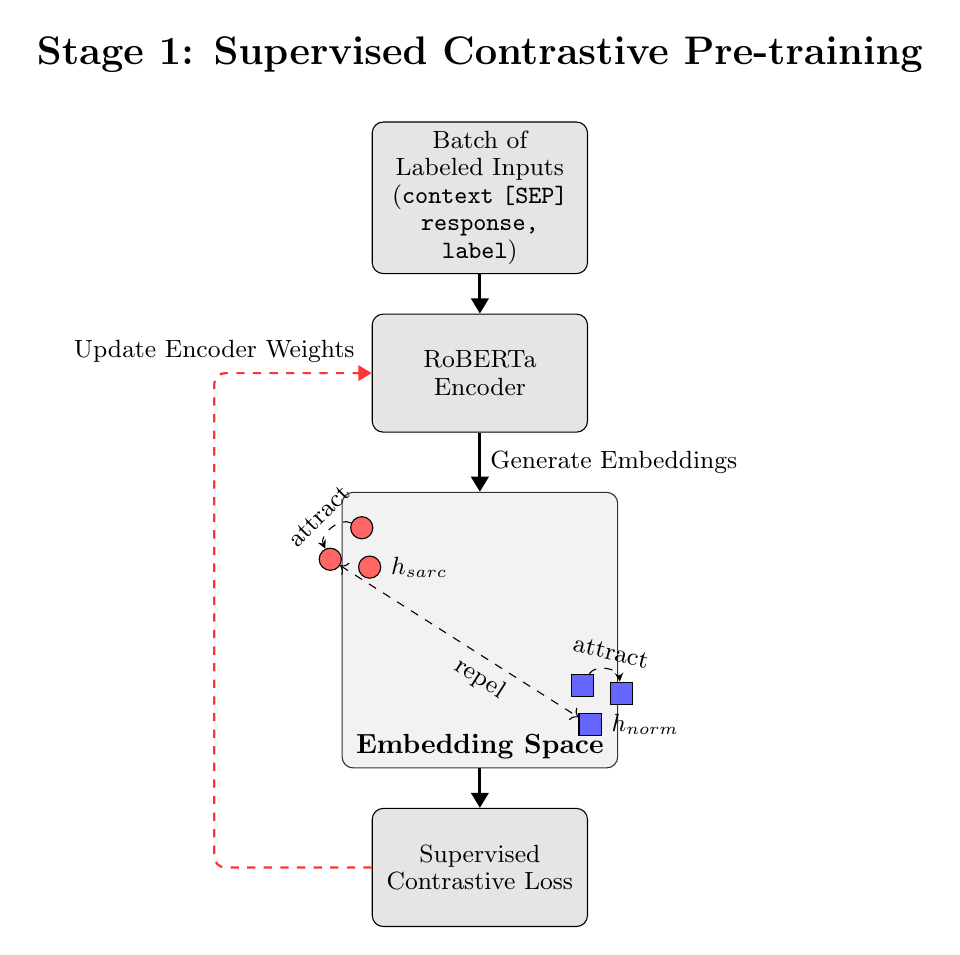
\begin{tikzpicture}[node distance=.5cm]

    % --- Title ---
    \node (title) [title] {Stage 1: Supervised Contrastive Pre-training};

    % --- Input Data ---
    \node (input) [block, below=of title] {Batch of Labeled Inputs \\ \small(\texttt{context [SEP] response, label})};

    % --- RoBERTa Encoder ---
    \node (encoder) [block, below=of input] {RoBERTa Encoder};
    \draw [main_arrow] (input) -- (encoder);

    % --- Embedding Space ---
    \node (emb_space) [space, below=.75cm of encoder] {};
    \node [above] at (emb_space.south) {\textbf{Embedding Space}};
    \draw [main_arrow] (encoder) -- (emb_space) node [midway, right, font=\small] {Generate Embeddings};

    % Coordinates for embedding clusters
    \coordinate (c1) at ($(emb_space.center)+(-1.5, 1.3)$); % Sarcastic cluster
    \coordinate (c2) at ($(emb_space.center)+(1.3, -0.7)$); % Not Sarcastic cluster

    % Sarcastic Embeddings (Circles)
    \node[sarc_emb] (s1) at (c1) {};
    \node[sarc_emb] (s2) at ($(c1)+(-0.4,-0.4)$) {};
    \node[sarc_emb, label={[font=\small]right:$h_{sarc}$}] (s3) at ($(c1)+(0.1,-0.5)$) {};

    % Not Sarcastic Embeddings (Squares)
    \node[norm_emb] (n1) at (c2) {};
    \node[norm_emb] (n2) at ($(c2)+(0.5,-0.1)$) {};
    \node[norm_emb, label={[font=\small]right:$h_{norm}$}] (n3) at ($(c2)+(0.1,-0.5)$) {};

    % Force arrows illustrating the contrastive objective
    \draw[force_arrow, black, bend right=70] (s1) to node[midway, above, sloped, font=\small] {attract} (s2);
    \draw[force_arrow, black, bend left=70] (n1) to node[midway, above, sloped, font=\small] {attract} (n2);
    \draw[force_arrow, black, <->] (s2) to node[midway, below right, sloped, font=\small] {repel} (n3);

    % --- Loss Function ---
    \node (loss) [block, below=of emb_space] {Supervised Contrastive Loss};
    \draw [main_arrow] (emb_space) -- (loss);

    % --- Weight Update Path ---
    \draw [update_arrow] (loss.west) -- ++(-2,0) |- (encoder.west)
    node [midway, above, font=\small] {Update Encoder Weights};

\end{tikzpicture}
        \caption{Overview of Stage 1: Supervised Contrastive Pre-training.}
        \label{fig:stage1}
    \end{figure}

    \subsubsection{Stage 2: Classification Fine-tuning}
    Figure~\ref{fig:stage2} details the second stage, where the model is fine-tuned for the binary classification task.
    The RoBERTa encoder is initialized with the weights optimized in Stage 1.
    In this stage, we switch to using the \texttt{[CLS]} token embedding, which is fed into a newly initialized linear classification head~\cite{khosla2020supervised}.

    The model outputs a prediction (``Pred'') which is compared against the ``True Label'' using a standard Cross-Entropy Loss.
    A critical component of this stage, visualized by the split update arrows in Figure~\ref{fig:stage2}, is the use of differential learning rates.
    The red arrows indicate that the classifier head is updated with a higher learning rate to rapidly learn the decision boundary, while the encoder is fine-tuned with a significantly lower learning rate.
    This strategy preserves the cluster structure learned in Stage 1 while allowing the model to adapt to the specific classification objective~\cite{moukafih2022simscl}.

    \begin{figure}[H]
        \centering
        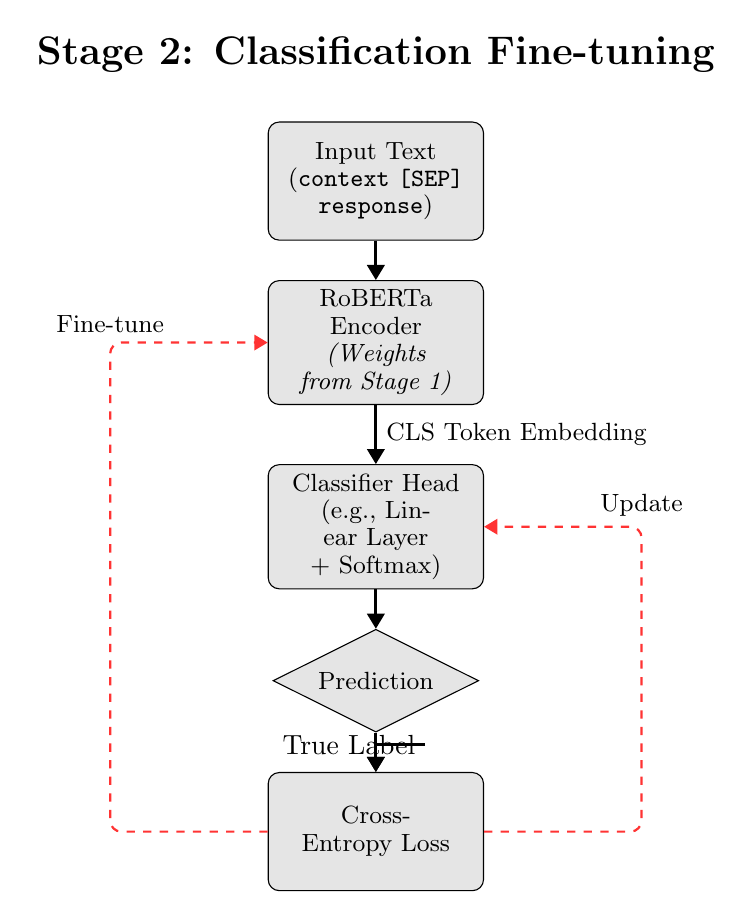
\begin{tikzpicture}[node distance=.5cm]

    % --- Title ---
    \node (title) [font=\Large\bfseries] {Stage 2: Classification Fine-tuning};

    % --- Input Data ---
    \node (input) [block, below=of title] {Input Text \\ \small(\texttt{context [SEP] response})};

    % --- RoBERTa Encoder ---
    \node (encoder) [block, below=of input] {RoBERTa Encoder \\ \small\textit{(Weights from Stage 1)}};
    \draw [main_arrow] (input) -- (encoder);

    % --- Classifier Head ---
    \node (classifier) [block, below=.75cm of encoder] {Classifier Head \\ \small(e.g., Linear Layer + Softmax)};
    \draw [main_arrow] (encoder) -- (classifier) node [midway, right, font=\small] {CLS Token Embedding};

    % --- Final Prediction ---
    \node (prediction) [output, below=of classifier] {Prediction};
    \draw [main_arrow] (classifier) -- (prediction);

    % --- Loss Calculation (Revised Style) ---
    \node (loss) [block, below=of prediction] {Cross-Entropy Loss};
    \draw [main_arrow] (prediction) -- (loss);

    % Replace the block with a simple text node for the label
    \node (label_text) [above left=0.1cm and -2cm of loss] {True Label};
    \draw [main_arrow] (label_text) -| (loss.north);

    % --- Weight Update Paths ---
    % Path to update the classifier (rerouted to the right)
    \draw [update_arrow] (loss.east) -- ++(2,0) |- (classifier.east)
    node [midway, above, font=\small] {Update};

    % Path to update the main encoder (originating from a clean point)
    \draw [update_arrow] (loss.west) -- ++(-2,0) |- (encoder.west)
    node [midway, above, font=\small] {Fine-tune};

\end{tikzpicture}
        \caption{Overview of Stage 2: Classification Fine-tuning.}
        \label{fig:stage2}
    \end{figure}

    \section{Experiments}

    \subsection{Datasets}
    We conducted our evaluation using the two primary datasets from the FigLang 2020 Shared Task on Sarcasm Detection~\cite{ghosh2020report}.
    Both datasets are balanced binary classification tasks and include conversational context.
    \begin{itemize}
        \item \textbf{FigLang-Reddit:} Comprises 4,400 training samples and 1,800 test samples.
        Sarcasm in this dataset is self-annotated by users via the \texttt{/s} tag.
        The dataset is characterized by longer conversation threads and complex discourse structures.
        \item \textbf{FigLang-Twitter:} Comprises 5,000 training samples and 1,800 test samples.
        Labels are derived from hashtags such as \#sarcasm and \#sarcastic.
        This dataset tends to feature shorter, more informal text with higher noise levels.
    \end{itemize}
    For our experiments, we partitioned the provided training data into a 90\% training set and a 10\% validation set to monitor convergence and perform model selection.

    \subsection{Experimental Setup}
    We benchmarked our SimSCLSD framework against a strong baseline to isolate the effect of contrastive pre-training.
    All experiments utilized the \texttt{roberta-base}~\cite{liu2019roberta} architecture with a batch size of 64.
    Early stopping was applied with a patience of 2 epochs based on validation Macro F1-score.

    \textbf{Baseline (Standard Fine-Tuning):} The model is fine-tuned directly on the target datasets using Cross-Entropy loss for up to 10 epochs.
    This represents the standard industry approach to text classification.
    Learning rates were tuned specifically for each dataset ($3 \times 10^{-5}$ for the classifier head; $5 \times 10^{-7}$ to $1 \times 10^{-6}$ for the encoder).

    \textbf{SimSCLSD (Ours):} During the first stage, the encoder is trained for 20 epochs using $\mathcal{L}_{\text{SupCon}}$ with a learning rate of $5 \times 10^{-5}$ and temperature $\tau=0.2$.
    In the second stage, The model is fine-tuned using CE loss for up to 10 epochs.
    We used differential learning rates: $3 \times 10^{-5}$ (Twitter) and $1 \times 10^{-5}$ (Reddit) for the classifier, and $5 \times 10^{-7}$ (Twitter) and $1 \times 10^{-6}$ (Reddit) for the encoder.
    Dropout was set to 0.1 for Twitter and 0.5 for Reddit to mitigate overfitting given the dataset sizes.

    \subsection{Results and Discussion}
    Table~\ref{tab:results} presents the performance metrics (Precision, Recall, and Macro F1) on the official test sets.
    The model checkpoint that performed best on the validation set was used for final testing.

    \begin{table}[H]
        \centering
        \caption{Performance comparison between the Baseline and the SimSCLSD framework on FigLang 2020 datasets. All metrics are Macro-averaged.}
        \label{tab:results}
        \begin{tabular}{l c c c c c}
            \toprule
            \textbf{Model} & \textbf{Dataset} & \textbf{Split} & \textbf{Precision} & \textbf{Recall} & \textbf{Macro F1} \\
            \midrule
            \multirow{2}{*}{Baseline} & \multirow{2}{*}{Reddit} & Dev & 0.5679 & 0.5568 & 0.5379 \\
            & & Test & 0.5244 & 0.5228 & 0.5148 \\
            \midrule
            \multirow{2}{*}{\textbf{SimSCLSD}} & \multirow{2}{*}{\textbf{Reddit}} & Dev & 0.6974 & 0.6955 & 0.6947 \\
            & & \textbf{Test} & \textbf{0.6166} & \textbf{0.6139} & \textbf{0.6116} \\
            \midrule
            \multirow{2}{*}{Baseline} & \multirow{2}{*}{Twitter} & Dev & 0.7352 & 0.7300 & 0.7285 \\
            & & Test & 0.7047 & 0.6861 & 0.6788 \\
            \midrule
            \multirow{2}{*}{\textbf{SimSCLSD}} & \multirow{2}{*}{\textbf{Twitter}} & Dev & 0.8486 & 0.8480 & 0.8479 \\
            & & \textbf{Test} & \textbf{0.7477} & \textbf{0.7461} & \textbf{0.7457} \\
            \bottomrule
        \end{tabular}
    \end{table}

    On the FigLang-Reddit dataset, SimSCLSD achieves a Macro F1-score of 0.6116, outperforming the baseline (0.5148) by a substantial margin of 9.68 percentage points.
    Similarly, on the FigLang-Twitter dataset, our method yields an F1-score of 0.7457 compared to the baseline's 0.6788, an improvement of 6.69 percentage points.

    These gains can be attributed to the nature of the contrastive loss.
    In sarcasm detection, the distinction between a sarcastic and a sincere statement often hinges on subtle semantic cues within the context.
    Standard CE training may struggle to separate these embeddings when the vocabulary overlap is high.
    By enforcing a compact clustering of sarcastic examples during pre-training, SimSCLSD essentially teaches the encoder to recognize the latent structure of sarcasm before it attempts to classify it, leading to a more robust decision boundary in the second stage.

    \section{Conclusion}
    In this paper, we introduced SimSCLSD, a two-stage framework for context-aware sarcasm detection that integrates supervised contrastive learning with transformer-based fine-tuning.
    We hypothesized that the widely used Cross-Entropy loss is suboptimal for nuanced linguistic tasks and that explicitly structuring the embedding space could yield better performance.

    Our extensive experiments on the FigLang 2020 shared task datasets validated this hypothesis.
    By preceding standard classification training with a supervised contrastive pre-training phase, we achieved statistically significant F1-scores improvements of 9.7\%p on the Reddit dataset and 6.7\%p on the Twitter dataset.
    This confirms that learning to discriminate between classes in the representation space provides a stronger foundation for the final classifier than learning the decision boundary alone.

    Future work could explore the applicability of this framework to larger architectures and investigate its generalization to other complex figurative language tasks, such as irony detection and metaphor identification.

% --- REFERENCES ---
    \bibliographystyle{IEEEtran}
    \bibliography{references}

\end{document}



